\vspace{1em}

\usetikzlibrary{graphs, positioning, quotes, shapes.geometric}

\begin{document}
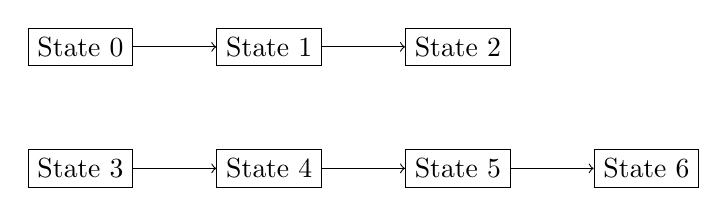
\begin{tikzpicture}[node distance=10pt]
    % 單純一條線,從initial state 到 finite state
    \node[draw]                           (State 0)  {State 0};
    \node[draw, right=30pt of State 0]    (State 1)  {State 1};
    \node[draw, right=30pt of State 1]    (State 2)  {State 2};
    
    \node[draw, below=30pt of State 0]    (State 3)  {State 3};
    \node[draw, right=30pt of State 3]    (State 4)  {State 4};
    \node[draw, right=30pt of State 4]    (State 5)  {State 5};
    \node[draw, right=30pt of State 5]    (State 6)  {State 6};

    \graph{
        (State 0) -> (State 1) -> (State 2);
        (State 3) -> (State 4) -> (State 5) -> (State 6);
    };
\end{tikzpicture}